% Add "answers" option to print the answers
\documentclass[addpoints]{exam}

\usepackage[utf8]{inputenc}
\usepackage{calc}
\usepackage[dvipsnames]{xcolor}
\usepackage{ifthen}
\usepackage{tcolorbox}

% \makebox[\textwidth]{Name:\enspace\hrulefill}
%  
% \vspace{5mm}
%\makebox[\textwidth]{Instructor’s name:\enspace\hrulefill}

\definecolor{MyLightGray}{gray}{0.60}

\newcommand{\truefalse}
{		\begin{checkboxes}
			 \choice True
			 \choice False. Explanation: 
		\end{checkboxes}
		\vspace{10pt}
}


% Check if 'answers' is an option
\newcommand{\ifanswers}[2]{%
  \ifthenelse{\boolean{exam@answers}}{#1}{#2}%
}



\newcommand{\answerspace}[1]
{
	\ifprintanswers
	\else
		\setlength{\mylength}{10pt}%
		% \vspace{#1\mylength}
		% Make the grey box
		\par\nobreak\noindent
		\makebox[\linewidth][l]{%
			% set inner padding to zero, so only the frame shows
			{\setlength{\fboxsep}{0pt}%
			% draw a color frame, white (or transparent) inside
			\fcolorbox{MyLightGray}{white}{%
			% the inner box has zero width content but fixed height
			\parbox[t][#1\mylength][c]{%
				% subtract twice the frame‐thickness from the full width
				\dimexpr\linewidth-2\fboxrule\relax
			}{\strut}%
			}%
			}%
		}%
		\par
		\vspace{3\mylength}

  	\fi
}
\newlength{\mylength}

\newcommand{\code}[1]{{\texttt{#1}}}

\newcommand{\answer}[1]{\begin{solution}{#1}\end{solution}}




%\usepackage{listings}
\usepackage{color}
\usepackage{lastpage}
\usepackage{verbatim}
\usepackage{fancyvrb}
\usepackage{graphicx}
\usepackage{float}
\usepackage{minted}

\usepackage{subcaption}

\usepackage{tikz}
\usetikzlibrary{positioning}

\usepackage[colorlinks=true, linkcolor=blue]{hyperref}

\newcommand{\includecode}[2][c]{\lstinputlisting[caption=, escapechar=, language=#1]{#2}<!---->}
\RecustomVerbatimCommand{\VerbatimInput}{VerbatimInput}{}

\newcommand{\Code}[1]{\mintinline{java}{#1}}
\newcommand{\ACC}[4]{\{\Code{x}$\mapsto$\Code{#1},
  \Code{y}$\mapsto$\Code{#2}, \Code{z}$\mapsto$\Code{#3}\}}


\renewcommand{\solutiontitle}{\noindent\textbf{Solution sketch: }}

\definecolor{SolutionColor}{rgb}{0.8,0.9,1}

\cfoot{Page \thepage\ of \pageref{LastPage}}

\rhead{Initials: \rule{20mm}{0.4pt}}



%%%%%%%%%%%%%%%%%%%%%%%%%%%%%%%%%%%%%%%%
\begin{document}
\fvset{numbers=left,numbersep=3pt}
\thispagestyle{empty}

\begin{center}
	{\LARGE CS 408 Spring 2026 -- Final (A)\\}

	\vspace{20mm}
\fbox{\fbox{\parbox{5.5in}{\centering
	\begin{itemize}
          % \item Write your \textbf{name} in the first page and your \textbf{initials in every other page}.
        \item The exam is closed notes, closed book.

        \item The exam should be completed individually: any
          communication with your fellow students is \textbf{strictly}
          prohibited.

	\item Please print or write legibly.

        \item If you have a question, raise your hand and the
          course staff will come to you.

        \item Provide complete and clear but concise
          answers. Any explanations should be thorough.

        \item Answer the questions in the spaces provided. Your answer
          does not need to take up all the space provided (hopefully
          we've given you more than enough room!). If you do run out
          of space, make a note and then use the empty pages at the
          back of the exam to complete your answer.

        \item Coding questions should be answered in Java, unless
          stated otherwise.

        \item Unless otherwise noted, CFG nodes represent basic blocks.
          % or low-level pseudo-code.
          % \item Unless otherwise noted, assume that questions refer to C code, AT\&T assembly syntax and the x86 architecture.

        \item Please double check that your copy of the exam
          is complete; you should have \pageref{LastPage}
          pages.

        \item You have 120 minutes to complete the exam.
        \end{itemize}
	}}}
\end{center}


\vspace{13mm}
\begin{center}
  \resizebox{0.8\textwidth}{!}{
    \combinedgradetable[h][questions]
  }
\end{center}
%\begin{center}\combinedgradetable[h][questions]\end{center}
\vspace{20mm}

\makebox[\textwidth]{\textbf{Name (please print)}: \rule{100mm}{0.8pt} }
%\end{center}

\vspace{10mm}
%\begin{center}
\makebox[\textwidth]{\textbf{PUID}: \rule{40mm}{0.8pt} \hspace{35mm}}
% \end{center}

\vspace{10mm}
%\begin{center}
\makebox[\textwidth]{\textbf{Ticket \#}: \rule{40mm}{0.8pt} \hspace{35mm}}
%\end{center}

\newpage
\begin{center}
  [PAGE DELIBERATELY LEFT BLANK]
\end{center}

\begin{questions}

  \newpage
  % \question State whether the following statements are true of false. \textbf{Explain the false statements.}
  %   \begin{parts}
  %   \part[2]
  %     \truefalse
  %     \answer{True.}
  %
  %   \end{parts}

  %  ## Topics: Fault versus error state versus failure

  %   Problem: Under the RIPR model, is it possible for a test case to
  %   trigger an error state without inducing a failure?

\question[1] %
  Under the RIPR model, is it ever possible for a test case to trigger
  an error state without inducing a failure? You may answer this
  question with a simple ``yes'' or ``no''. %
  \answerspace{5} %

  %   Problem: Under the RIPR model, can a test case ever induce a
  %   failure if the program under test does not
  %   have a fault?

\question[1] %
  Under the RIPR model, if the program under test does not contain a
  fault, can a test case ever induce a failure? Again, an answer of
  ``yes'' or ``no'' will suffice.
  \answerspace{5} %

% ## Syntactic Coverage Critera:

\question[3] %
  Order the following CFG-based coverage criteria using the
  subsumption relation: (A) edge coverage, (B) prime path coverage,
  (C) node coverage, (D) complete path coverage. Your answer should
  have the form: A $\supseteq$ B $\supseteq$ C $\supseteq$ D, where A
  subsumes B, B subsumes C, and C subsumes D.

  \answerspace{10} %

\question[2] %
  For an arbitrary program, is it always possible to find a test set
  that achieve 100\% node coverage for that program? If your answer is
  ``yes'', explain why in 2-3 sentences. If your answer is ``no'',
  provide a short ($\leq$ 5 line) program for which 100\% node
  coverage is impossible.

  \answerspace{15} %

\newpage
\begin{center}
  [PAGE DELIBERATELY LEFT BLANK]
\end{center}
\newpage

% \begin{parts}
% \part[3]  %
%   \answerspace{15} %
%   \begin{solution}
%   \end{solution}
% \end{parts}

% ## Logic Coverage Criteria

\question Consider the following Java program:
  \vspace{-.3cm}
  \begin{minted}{java}
int foo(int x, char y, int z) {
  int out = 0;
  if (z > 0 || (x < -10 && y == 'y')) {
    out = 1;
  } else {
    out = 2;
  }
return out;
}
\end{minted}
\begin{parts}

\part[2] Give a minimal test set that achieves 100\% predicate
  coverage for \Code{foo}. If this is not possible,
  explain why in 2-3 sentences. %
  \answerspace{17} %
  \begin{solution}
    We only need two test cases, one in which the first clause is
    \Code{true}, e.g. \ACC{0}{'0'}{1}, and another in which the first
    clase is \Code{false}, e.g, \ACC{0}{'0'}{-1}.
  \end{solution}

\part[2] Give a test set that achieves 100\% clause coverage but
  \textit{not} 100\% predicate coverage for \Code{foo}. If
  this is not possible, explain why in 2-3 sentences. %
  \answerspace{17} %
  \begin{solution}
    Here, we can acheive this with the following test set:
    \ACC{0}{'0'}{1}, \ACC{-20}{'y'}{0}.
  \end{solution}

\newpage
\begin{center}
  [PAGE DELIBERATELY LEFT BLANK]
\end{center}
\newpage

\part[5] Give a test set that achieves 100\% Generalized Active Clause
  coverage (GACC) but \textit{not} 100\% predicate coverage for
  \Code{foo}. If this is not possible, explain why in 2-3 sentences. %
  \answerspace{20} %

  \begin{solution} This is not possible. To achieve 100\% GACC, we
    need a pair of tests in which \Code{x < -10} is an
    active clause; one of these needs to make the clause
    \Code{true} and another needs to make it %
    \Code{false}. We have no freedom to pick the truth
    values for the other clauses, though: there is exactly one
    scenario where the \Code{x < -10} clause determines
    this predicate, i.e., when \Code{z > 0} is
    \Code{false} and %
    \Code{y == 'y'} is \Code{true} (a similar
    argument applies to the \Code{y == 'y'} clause). Under
    this assignment, the truth of the predicate is completely
    determined by \Code{x < -10}: any test that makes
    \Code{true} makes the predicate
    \Code{true}, and any test that makes the clause
    \Code{false} similarly makes the predicate
    \Code{false}, thus guaranteeing 100\% predicate
    coverage for \Code{foo}.
    % \VerbatimInput{midterm-q7_d_answer.txt}
  \end{solution}
\end{parts}

% ## Concolic Execution:

\vspace{-.3cm}
\question[1] Name one advantage that concolic execution has compared
  to coverage-guided greybox fuzzing. %
  \answerspace{12} %
  \begin{solution}
    A concolic execution engine typcially assumes complete access to
    the program under test, so it can guarantee a new path will be
    explored with each new test it generates. Coverage-guided fuzzers
    offer no such guarantee. \\
    In general, any answer that shows the student knows that concolic
    execution is a white-box approach and that they are able to
    compare and contrast grey- and white-box testing approaches works
    here.
  \end{solution}

  \vspace{-.3cm}
\question[1] Name one disadvantage that concolic execution has
  compared to coverage-guided greybox fuzzing. %
  \answerspace{12} %
  \begin{solution}
    A concolic execution engine requires access to the source code of
    the system under test. It also requires a solver to find new
    inputs, which can be slow and may not work if the system under
    test uses complicated path conditions. \\ %
    As with the previous question, any answer that shows the student
    knows that concolic execution is a white-box approach and that
    they are able to compare and contrast grey- and white-box testing
    approaches works here.
  \end{solution}


\newpage
\begin{center}
  [PAGE DELIBERATELY LEFT BLANK]
\end{center}
\newpage

\question Consider the following Java program:
  \vspace{-.3cm}
  \begin{minted}{java}
int bar(int[] a) {
  int s = 0;
  if (a.length < 3) return;
  for (int i = 0; i < 3; i++) {
    if (a[i] >= i) {
      s = s + a[i];
    } else {
      s = s - a[i];
    }
  }
  if (s % 2 == 0) {
    return 1;
  } else {
    return 0;
  }
}
\end{minted}
\begin{parts}

\part[6]
  List the final path constraint that concolic execution would produce
  for the program \Code{bar} on the test input
  $a = [1, 0, 3]$. Give your answer as a sequence of path conditions
  separated by $\land$, e.g., for the path conditions $P$, $Q$, and
  $R$, write $P \land Q \land R$ . When writing your path condition,
  assume the initial symbolic input has the form
  $arr \mapsto [a , b, c]$, and write the symbolic value stored at
  index $0$ as $a$, $1$ as $b$, and $2$ as $c$. You are allowed to
  drop clauses that are always true, e.g., $3 < 5 + 1$ from the path
  constraint, but otherwise you should not simplify it in any way.
  \answerspace{15} %
  \begin{solution}
    Final path constraint is: $\lnot$ \Code{a.length < 3} $\land$
    \Code{a >= 0} $\land$ $\lnot$ \Code{b >= 1} $\land$ \Code{c >= 2} $\land$
    \Code{(a - b + c)} \Code{\% 2 == 0}
    \end{solution}
  \vspace{-.7cm}
\part[3] List the next two new inputs that a concolic execution engine
  might generate after executing \Code{bar} on the test
  input $[1, 0, 3]$. %
  \answerspace{11} %
  \begin{solution}
    Anything that flips the last path constraint they had above will
    work. Assuming they correctly generated the path condition in the
    previous part, we need an array with three elements whose first
    element is greater than -1, second element is less than 1, third
    element is greater than 1, and whose first three elements sum up
    to an odd number, e.g.,  $arr \mapsto$ \Code{[1, 0, 2]}. \\
    For the second input, we need an array whose third element is less
    than 2, e.g., $arr \mapsto$ \Code{[1, 0, 1]}.
  \end{solution}
\end{parts} %
%
\newpage
\begin{center}
  [PAGE DELIBERATELY LEFT BLANK]
\end{center}
\newpage

  % ## Test Oracles:

\question[2] Which category of test oracle discussed in class would an
  off-the-shelf blackbox fuzzer typically use? Explain your answer in
  2-3 sentences.

  \answerspace{20} %
  \begin{solution}
    An implicit oracle is the standard, because it works 'out of the
    box' on an arbitrary program, and greybox fuzzers are typically
    designed to be as push-button as possible.
  \end{solution}

\question[2] In 2-4 sentences, describe an automated testing scenario
  where a blackbox fuzzer might use a different kind of test oracle
  discussed in class. Be sure to explicitly state which category of
  test oracle is used, and to justify why it is reasonable to use in
  this scenario.

  \answerspace{20} %

  \begin{solution}
    There are many possible answers here. The key thing is that they
    need to identify a particular application which enable us to use a
    more intelligent test oracle: e.g. when fuzzing an image
    processing algorithm we can use a metamorphic relation as an
    oracle, or when fuzz testing a compiler optimization we can use a
    reference implementation as an oracle.
  \end{solution}


\newpage
\begin{center}
  [PAGE DELIBERATELY LEFT BLANK]
\end{center}
\newpage

  % ## Delta Debugging:

\question Suppose that we have the test input
  $[1, 2, 3, 5, 3, 8, 7, 10, 42, 11]$, and a sorting program that
  fails if and only if it is given a list with at least two elements,
  one of which is the number $3$, and which contains at least one pair
  of adjacent elements where the first element is greater than the
  second. Identify which of the following test inputs would be
  considered as a possible test case by the delta debugging algorithm
  (\Code{ddmin}) discussed in class, noting whether or not
  each is a valid final output of \Code{ddmin}. (Indicate
  your answer by circling your choice.)

  \begin{parts}
  \part[2] $[1, 2, 3, 5, 3]$
    \begin{itemize}
    \item[ ] Considered by \Code{ddmin}: Yes \quad/\quad No %
      \hfill Valid Output of \Code{ddmin}: Yes \quad/\quad No
    \end{itemize}
    \vspace{12pt}

  \part[2] $[1, 3, 8, 10]$
    \begin{itemize}
    \item[ ] Considered by \Code{ddmin}: Yes \quad/\quad No %
    \hfill Valid Output of \Code{ddmin}: Yes \quad/\quad No
  \end{itemize}
  \vspace{12pt}

  \part[2] $[3, 7, 8]$
    \begin{itemize}
    \item[ ] Considered by \Code{ddmin}: Yes \quad/\quad No %
    \hfill Valid Output of \Code{ddmin}: Yes \quad/\quad No
  \end{itemize}
  \vspace{12pt}

  \part[2] $[5, 3]$
    \begin{itemize}
    \item[ ] Considered by \Code{ddmin}: Yes \quad/\quad No %
    \hfill Valid Output of \Code{ddmin}: Yes \quad/\quad No
  \end{itemize}
  \vspace{12pt}

    \part[2] $[3, 6]$
    \begin{itemize}
    \item[ ] Considered by \Code{ddmin}: Yes \quad/\quad No %
    \hfill Valid Output of \Code{ddmin}: Yes \quad/\quad No
    \end{itemize}
  \end{parts}
  \vspace{24pt}

%   % ## Regression Testing

% \question[3] Identify two challenges related to regression testing
%   that were discussed in class. For each challenge, describe a
%   concrete mitigation strategy and provide 1-2 sentences explaining
%   how they address the issue.

%   \begin{itemize}
%   \item \textbf{Challenge \#1:}\\
%     \fbox{
%       \begin{minipage}{.95\linewidth}
%         \hfill
%         \\[24pt]
%       \end{minipage}
%     }
%   \item \textbf{Mitigation Strategy \#1:} \\
%     \fbox{
%       \begin{minipage}{.95\linewidth}
%         \hfill
%         \\[84pt]
%       \end{minipage}
%     }
%     \\
%   \item \textbf{Challenge \#2:}\\
%     \fbox{
%       \begin{minipage}{.95\linewidth}
%         \hfill
%         \\[24pt]
%       \end{minipage}
%     }

%   \item \textbf{Mitigation Strategy \#2:} \\
%     \fbox{
%       \begin{minipage}{.95\linewidth}
%         \hfill
%         \\[84pt]
%       \end{minipage}
%     }
%   \end{itemize}

  % ## Static versus Dynamic Analysis (Practice Exam):

\question[4] Classify each of the following program analysis as either
  Dynamic or Static. (Indicate your answer by circling your choice.) \\

  \begin{itemize}
  \item \textbf{Concolic Execution}: Dynamic \quad/\quad Static
    \\[24pt]
  \item \textbf{Lockset Analysis}: Dynamic \quad/\quad Static
    \\[24pt]
  \item \textbf{Path-Insensitive Data-Flow Analysis}: Dynamic \quad/\quad Static
    \\[24pt]
  \item \textbf{Black-Box Randomized Testing}: Dynamic \quad/\quad Static \\[24pt]
  \end{itemize}

  \newpage
\begin{center}
  [PAGE DELIBERATELY LEFT BLANK]
\end{center}
\newpage

  % ## Static Analysis:

\question[10] Show the annotated CFG that results from performing sign
  analysis on the function \Code{baz} (\autoref{fig:baz})
  using the path-insensitive, forward data-flow analysis over the sign
  domain, using the algorithm discussed in class.For reference, we've
  given the Hasse diagram for the sign domain you should use in
  \autoref{fig:sign+domain}. Your analysis should use
  \Code{[y }$\mapsto \top, $%
  \Code{x }$\mapsto \bot, %
  $\Code{z }$\mapsto \bot$\Code{]} for the
  input abstract state. Your answer should be given in the form of a
  CFG, where each node of the CFG is annotated with an input abstract
  state, basic block / conditional identifier, and an output abstract
  state. In order to receive partial credit, an answer should at least
  provide the correct CFG structure for \Code{baz}, even
  if its input and output state annotations are incorrect.%
  \begin{figure}[ht]
    \begin{subfigure}{.45\linewidth}
      \begin{center}
  \begin{minted}{java}
int baz(int y) {
  int x = 0;
  int z = 0;
  while (y > 0) {
    if (x >= 0) {
      x = x + 1;
    } else {
      x = 1;
    }
    y = y - 1;
  }
  if (x >= 0) {
    z = 1;
  } else {
    z = -2;
  }
  return z;
 }
\end{minted}
      \end{center}
      \caption{A rather silly Java program}
      \label{fig:baz}
    \end{subfigure}
    \begin{subfigure}{.3\linewidth}
      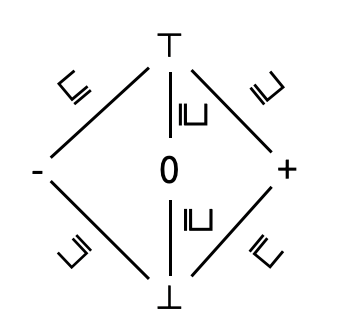
\includegraphics[width=.75\linewidth]{SignLattice.png}
      \caption{The Hasse diagram for the sign domain}
      \label{fig:sign+domain}
    \end{subfigure}
\end{figure}

  \answerspace{26}%
  %   Problem: Do a simple static sign analysis on a program.

  %   Part a: draw the CFG of this program.

  % Part b: annotate the CFG with the results of performing the static
  % analysis.

  \newpage
\begin{center}
  [PAGE DELIBERATELY LEFT BLANK]
\end{center}
\newpage

\if 0 %%%%%%%%%%%%%%%%%%%%%%%%%%%%%%%%%%%%%%%%%
	\question[10]
	\answerspace{30}
	\begin{solution}
          	\end{solution}

	\question
	\begin{parts}
		\part[6]
		\answerspace{20}
		\begin{solution}
                  	\end{solution}

		\part[2]
		\answerspace{10}
		\begin{solution}
                \end{solution}

	\end{parts}
\fi %%%%%%%%%%%%%%%%%%%%%%%%%%%%%%%%%%%%%%%%%

	\newpage
	\begin{center}
		[EMPTY PAGE 1 -- Use as overflow to complete your
                answers ]
	\end{center}

	\newpage
	\begin{center}
		[EMPTY PAGE 2 -- Use as overflow to complete your
                answers ]
              \end{center}

\end{questions}





\end{document}
